\documentclass{article}
\usepackage{fullpage}
\usepackage{mathpazo}
\usepackage{microtype}
\usepackage{graphicx}
\usepackage{wrapfig}
\usepackage{amsmath}

\newcommand\myfrac[2]{#1/#2}
\begin{document}

\noindent {\Huge\bf Gizmo}\\
{\large \bf An Arduino MIDI Tool\\
By Sean Luke\quad sean@cs.gmu.edu}\\
\\

\noindent Gizmo is a small MIDI device intended to be inserted between the MIDI OUT of one device and the MIDI IN of one or more other devices.  There are a number of tools like this, such as the esteemed MIDIPal \footnote{MIDIPal is quite similar to Gizmo in functionality and goals, but I wasn't even aware of the existence of MIDIPal when I started building Gizmo.  And besides, re-inventing the wheel is fun!  MIDIPal's page is http:/\!/mutable-instruments.net/midipal\ \ This device has been discontinued, but its open source software lives on in other hardware clones, such as the MIDIGal (https:/\!/midisizer.com/midigal/)  } or the variety of tools from MIDISolutions\footnote{http:/\!/www.midisolutions.com/}

Gizmo is the unholy union of an Arduino Uno or Arduino Mega 2560,\footnote{http:/\!/arduino.cc} an Adafruit 16x8 I2C LED matrix\footnote{https:/\!/www.adafruit.com/categories/326\quad I use the 1.2-inch 16x8 matrix with red round LEDs, which works well.  This particular model can be found at https:/\!/www.adafruit.com/products/2037}, and a SparkFun MIDI Shield\footnote{https:/\!/www.sparkfun.com/products/12898} to perform a variety of helpful MIDI tasks.  Gizmo has several built-in applications, and assuming there's space\footnote{On the Uno there's basically no extra space: we're at the limit.  So if you want to do an application you really should use a Mega.} you can develop additional applications for it.

This is a software project: the hardware is just three off-the-shelf boards and four wires.  There's no enclosure, no custom board.  If you'd like to do that, I'd welcome seeing it.

Gizmo comes built-in with the following applications and other capabilities:

\paragraph{Applications}
\begin{itemize}
\item {\bf Arpeggiator.}  Gizmo's arpeggiator has built-in up, down, up/down, repeated chord, and random arpeggios spanning one to three octaves.  Additionally, you can define up to ten additional arpeggiator patterns, each up to 32 notes long, involving up to 15 different chord notes, plus rests.  Arpeggios can be {\it latched} (or not), meaning that they may continue to play even after you have released the keys.  You can specify  the note value relative to the tempo (ranging from eighth triplets to double whole notes), the note length as a percentage of the note value (how legato or staccato a note is), the output MIDI channel, and the degree of swing (syncopation).  Gizmo will show the arpeggio on-screen.
\item {\bf Step Sequencer.}  Gizmo's step sequencer can be organized as 12 16-note tracks, 8 24-note tracks, or 6 32-note tracks.  Each note in a track can have its own unique pitch and velocity, or be a rest, or continue (lengthen, tie) the previous note.  You can also fix the velocity for an entire track, mute tracks, fade their volume, specify their independent output MIDI channels, specify the note value relative to the tempo (again ranging from eighth triplets to double whole notes), the note length as a percentage of the note value (how legato or staccato a note is), and the degree of swing (syncopation).    The step sequencer lets you edit in two modes: either by triggering independent steps like a classic drum sequencer, or by playing a sequence of notes.  The Arduino Uno can store up to two sequences in its slots (shared with the Recorder, discussed next).  The Mega can store up to nine sequences.  Gizmo will show and edit sequences on-screen.
\item {\bf Recorder.}  The Arduino doesn't have a lot of memory, but we provide a note recorder which records and plays back up to 64 notes (pitch and velocity) played over 21 measures. The recorder has 16-voice polyphony.   It's enough to record a very short ditty.  You can also set the recorder to loop the recording while playing, and to provide a click track.  The Arduino Uno can store up to two recordings in its slots (shared with the Step Sequencer).  The Mega can store up to nine recordings.
\item {\bf MIDI Gauge.}  The gauge will display all incoming MIDI information on one or all channels.  Note on, note off, and polyphonic aftertouch are shown with pitch and velocity (or pressure).  Channel aftertouch is shown with the appropriate pitch.  Program changes indicate the number.  Pitch bends indicate the value in full 14-bit.  Channel control, NRPN, and RPN messages display the number, value, and whether the value is being set, incremented, or decremented.  Sysex, song position, song select, tune request, start, continue, stop, and system reset are simply noted.  Rapid-fire MIDI signals such as MIDI clock, active sensing, and time code just turn on individual LEDs.
\item {\bf MIDI Control Surface}.  Gizmo has two potentiometers and two buttons.  Each can be configured to send a unique Program Change, Control Change, NRPN, or RPN commands, or optionally to output voltage values via either of two DACs.  The potentiometers can only send MSB values.
\end{itemize}

\paragraph{Other Cool Stuff}

As if this weren't enough, Gizmo also comes with the following capabilities.  All of these settings are automatically saved permanently in memory.

\begin{itemize}
\item {\bf Tempo and the MIDI Clock.}  Gizmo can sync to an external MIDI clock, can ignore it and use its own internal clock, and can emit the same as a MIDI clock.  Gizmo can also pass the external MIDI clock through or block it.  When using its own internal clock, Gizmo supports tempos ranging from 1 to 1024 BPM.  Gizmo applications can also be set with a {\it note value} (or {\it note speed}) to play their notes relative to this clock, ranging from eighth triplets (1/24 beat) to double whole notes (8 beats).  At any time, Gizmo pulses on-screen LEDs indicating the clock and note speed pulses.  Finally, Gizmo can be configured to vary the degree of {\it swing} or {\it syncopation}.

\item {\bf In and Out MIDI Channels}  Gizmo can be configured with input and output MIDI channels (some applications will use these: others will have multiple channels and will treat these as defaults).  Both channels can be turned off, and the input channel can be OMNI.  Gizmo pulses on-board LEDs indicating incoming and outgoing MIDI data.  

\item {\bf Remote Control via MIDI NRPN.} Gizmo can be controlled remotely via NRPN rather than using its on-board controls.  If you start using the controls, Gizmo's onboard potentiometers are locked out so their noise will not interfere with your remote control.  You can unlock the potentiometers by pressing a button on-board Gizmo, or by sending Gizmo's {\it Release} NRPN message.

\item {\bf Transposition and Volume Control}  You transpose all of Gizmo's MIDI output pitch by anywhere from \(-60...60\) steps.  Additionally you can multiply the MIDI output velocity (volume) by multiples of two ranging from \(1/8\) to \(8\).

\item {\bf Bypass.}  You can quickly put Gizmo in Bypass mode, to pass through all MIDI signals and generate no new ones.

\item {\bf Screen Brightness and Menu Delay}  You can change the screen brightness.  Also, many of Gizmo's menus display the first few letters of a menu item, then pause for some interval of time before they start scrolling the full item.  You can change this interval.

\end{itemize} 

\paragraph{Future Stuff (on the Arduino Mega)}

I have written but not tested some additional code.  It won't appear on the Uno version (not enough space) but may show up on the Mega version.  This stuff includes:

\begin{itemize}
\item {\bf Control Voltage}  You can configure Gizmo to optionally output voltage values from 0--5V, through two DACs, in response to notes being played.    One voltage output is in response to the note pitch, and the other is in response to the note velocity.  This would allow you to control non-MIDI devices which respond instead to voltage.

\item {\bf Per-MIDI Device Options}  There will be an area for specific kinds of MIDI devices.  For example, I have written code to convert NRPN values into the unusual sysex messages required by the Kawai K4 Synthesizer so it can be manipulated easily via a standard MIDI controller.

\item {\bf Keyboard Splitting}  You can split incoming MIDI notes by pitch and route them to different MIDI out channels.

\end{itemize}

Hopefully there'll be more than this.  Message filtering?  A MIDIPal-style CC LFO?  Longer note recorder songs?  And so on.

\section{Building Gizmo}

\begin{enumerate}

\item {\bf Assemble the Hardware}\quad Gizmo consists of an Arduino Uno or Arduino Mega, a SparkFun MIDI Shield\footnote{https:/\!/www.sparkfun.com/products/12898} attached via four wires (I2C) to an Adafruit 16x8 LED Matrix.\footnote{This matrix comes in various colors LED shapes (round, square), and matrix sizes (0.8 inch, 1.2 inch).  I personally use a 1.2 inch round red matrix.  The URL for my model is https:/\!/www.adafruit.com/products/2037}  The SparkFun MIDI Shield does not come with headers to plug into the Arduino, and you'll need to get those too: it's assumed you'll either use plain headers, or use stackable headers.  I use stackable headers as it makes it easy for me to plug my four test wires into it.

Attach the four wires for SDA, SCL, 5V, and GND between the MIDI Shield and the LED Matrix.  

\item {\bf Modify your Arduino Software}\quad You will need a pretty recent version of the Arduino software, as newer versions have better compilers which compile more compact code.  I developed Gizmo on Arduino 1.6.12 for MacOS X.  You will want to modify the source code files for the Arduino libraries in two spots:

\paragraph{Add Nonblocking I2C Writes}  This will dramatically speed up I2C for our purposes.
\begin{enumerate}
\item Locate your \texttt{Wire.cpp} and \texttt{Wire.h} files.  On the Mac they're located in\\\texttt{Arduino.app/Contents/Java/hardware/arduino/avr/libraries/Wire/src/}

\item Add the following line inside the ``public'' method region in \texttt{Wire.h:}

\begin{verbatim}
    uint8_t endTransmissionNonblocking();
\end{verbatim}

\item Add the following method to \texttt{Wire.cpp}:

\begin{verbatim}
    uint8_t TwoWire::endTransmissionNonblocking()
        {
        uint8_t ret = twi_writeTo(txAddress, txBuffer, txBufferLength, 0, 1);
        return ret;
        }
\end{verbatim}
\end{enumerate}

\paragraph{Reduce the I2C Buffer Size from 32 to 20} This gives us some extra static RAM space.

\begin{enumerate}
\item Locate your \texttt{Wire.h} file.  Again, on the Mac it's located in\\
\texttt{Arduino.app/Contents/Java/hardware/arduino/avr/libraries/Wire/src/}

\item Change the \texttt{BUFFER\_LENGTH} constant in the \texttt{Wire.h} file as follows:

\begin{verbatim}
        #define BUFFER_LENGTH 20   // Was 32
\end{verbatim}

\item Identify your \texttt{twi.h} file.  On the Mac it's located in\\
\texttt{Arduino.app/Contents/Java/hardware/arduino/avr/libraries/Wire/src/utility/}

\item Change the \texttt{TWIBUFFER\_LENGTH} constant in the \texttt{twi.h} file as follows:

\begin{verbatim}
        #define TWI_BUFFER_LENGTH 20    // Was 32
\end{verbatim}
\end{enumerate}

\item {\bf Install the FortySevenEffects MIDI Library}\quad But not straight off of its website.\footnote{https:/\!/github.com/FortySevenEffects/arduino\_midi\_library}  The MIDI library is in a state of flux and is having some significant additions being made.  The Gizmo code is extremely sensitive to code size (at least on the Uno).  Thus for now, use the version I include in Gizmo's Github repository.

\item {\bf Switch the MIDI Shield to ``Prog''}

\item {\bf Build and Upload Gizmo's Code to the Arduino}\quad  It should compile cleanly for either an Arduino Uno or an Arduino Mega 2560.  On the Uno it'll complain of Low Memory.

\item {\bf Switch the MIDI Shield to ``Run''}\quad  You can plug in MIDI cables now.

\item {\bf Reset Gizmo}\quad Power up the Arduino.  Then hold down all three pushbuttons on the MIDI Shield.  While doing so, press and release the reset button on the MIDI Shield.  Continue to hold down the three push buttons until the two LEDs on the MIDI Shield light up.  Let go of the pushbuttons.  

This procedure initializes the memory, options, and files in the device.  Now you're ready to go!

\end{enumerate}

\section{User Interface}

\begin{wrapfigure}{r}{3in}
\vspace{-1.5em}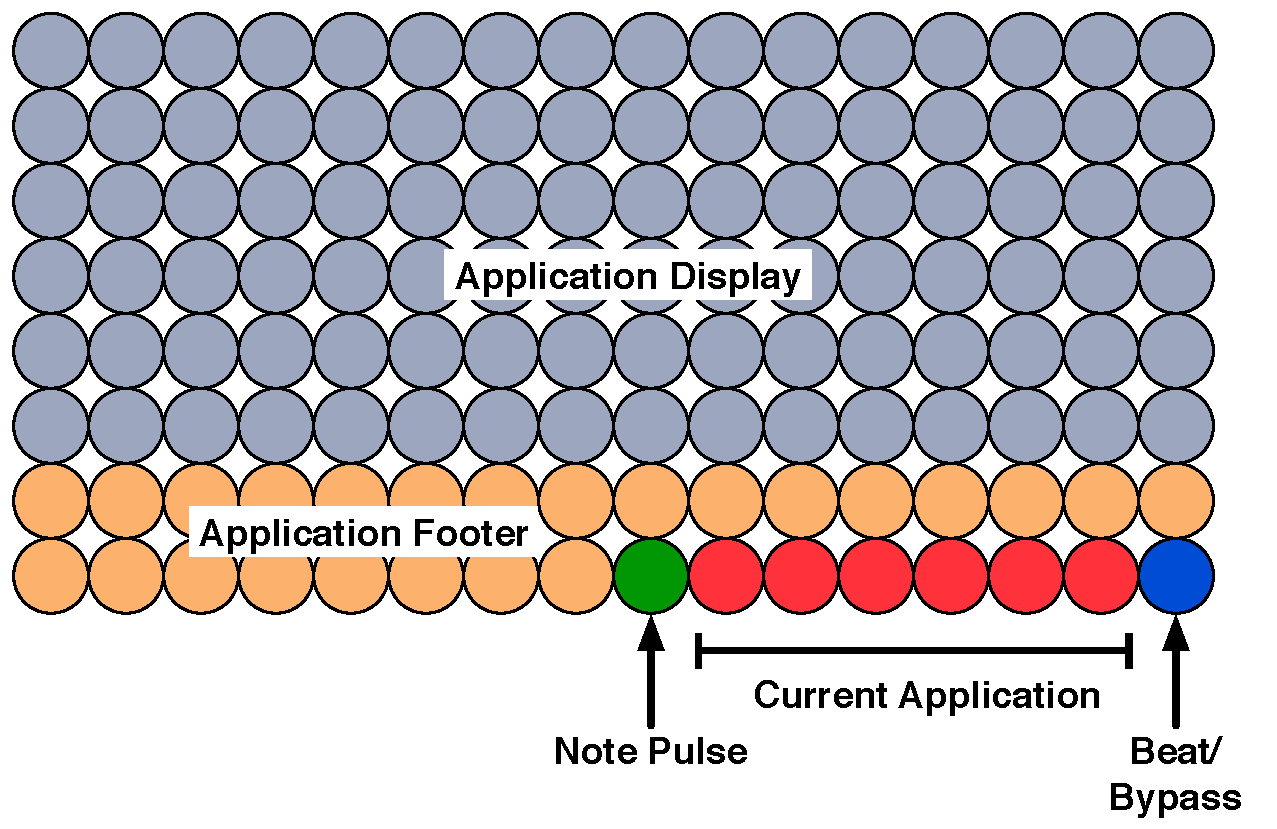
\includegraphics[width=3in]{OverallLayout.pdf}
\vspace{-2em}\caption{\small High-Level Gizmo Layout}\vspace{-2em}
\label{HighLevelGizmoLayout}
\end{wrapfigure}

Gizmo has a modest interface: a 16x8 LED display, two additional on-board LEDs (red and green), three buttons, and two potentiometers (dials): but it strives hard to make good use of these.  

Gizmo's top-level interface layout is a menu hierarchy.  You select menu items, which may take you deeper into the hierarchy, or you can go back up towards the top of the hierarchy.  The top level menu chooses between different {\bf applications}.  Once you have entered an application, its {\bf application number} is displayed in the {\bf current application region} (see Figure \ref{HighLevelGizmoLayout}).

\begin{wrapfigure}{r}{1.6in}
\includegraphics[width=1.6in]{Application.pdf}
\vspace{-2em}\caption{\small Application Values}\vspace{-2em}
\end{wrapfigure}

The current application LEDs light up right-to-left in a certain pattern with increasing application numbers, as shown in the figure at right.  Gizmo's interface can presently support up to eleven top-level applications.  

Also shown in Figure \ref{HighLevelGizmoLayout} are the {\bf Beat/Bypass} light and the {\bf Note Pulse} light.  The Beat/Bypass turns on and off every {\it beat} (quarter note).  This shows the current {\bf tempo}.\footnote{A beat occurs every 24 {\it pulses} of a MIDI Clock or Gizmo's internal clock.}  The Note Pulse light turns on and off every {\it note pulse}: this is the speed you have chosen for the arpeggiator, step sequencer, etc.  Note pulses are defined in terms of note value: for example, if the note pulse is presently in sixteenth notes, then this light will turn on and off four times faster than the beat light, which is in quarter notes. The note pulse light is also affected by the degree of swing (syncopation) you have defined.

The reset of the screen is given over to the application.  In many cases an application will display text and other data in the {\bf Application Display} region, while lighting up certain status LEDs in the {\bf Application Footer}.

You wend your way through menus, choose applications, and manipulate them using Gizmo's three buttons and two potentiometers as follows:

\paragraph{Buttons}  The left button is called the {\bf back button}.  The right button is called the {\bf select button}.  The center button is called (unsurprisingly) the {\bf middle button}.   The buttons respond to being {\bf pressed} and immediately released, and also respond to {\bf long presses}: holding a button down for a long time (presently one-half second) and then releasing it. 

Buttons do different things.  Here are certain common items:

\begin{itemize}
\item {\bf Pressing the Back Button}\quad This is the ``escape'' or ``cancel'' button: it {\bf always goes back up the menu hierarchy.}  Thus you can't ever get lost\,---\,just keep pressing the Back button and you'll eventually find yourself at the root menu.
\item {\bf Long-Pressing the Back Button}\quad This toggles {\bf bypass mode}, where Gizmo tries hard to act as if it's just a coupler between its input and output MIDI wires.  In bypass mode, the {\bf Beat/Bypass} light (Figure \ref{HighLevelGizmoLayout}) will stop beating and instead will flash rapidly.
\item {\bf Pressing the Select Button}\quad If you're being presented with a menu of options, or a number to choose, or a glyph to choose, the Select button will select the currently-displayed option.  In some applications (such as the Step Sequencer, Arpeggiator, and Recorder) the Select Button is assigned other tasks.
\end{itemize}

\paragraph{Potentiometers}

Gizmo's potentionmeters  (or {\bf pots}) do a number of tasks, including scrolling through menu options, moving a cursor horizontally or vertically, or choosing a number.  The left pot does primary tasks, and the right pot assists when appropate.  Note that these are potentiometers, not encoders: if you start turning one, you may experience a big jump initially.  The potentiometers have a limited range (0...1023), and a significant degree of noise, so realistically they can only choose numbers between 0...256 or so.  If asked to select a {\it big} number, the {\bf left pot} will act as a coarse-level selector, and the {\bf right pot} will fine-tune the number.


\paragraph{On-Board LEDs}

There are two LEDs on-board the SparkFun MIDI Shield.  The {\bf red LED} is toggled on and off to reflect incoming MIDI data.  The {\bf green LED} is toggled on and off to reflect outgoing MIDI data.  

\section{Initializing Gizmo}

Gizmo must be initialized before it can be used.  You can also do a factory reset on Gizmo with this procedure:

\begin{enumerate}
\item Hold down all three buttons
\item Press the reset button
\item Continue to hold down all three buttons until both on-board LEDs have lit.
\item Let go of the buttons.
\end{enumerate}

Gizmo will reset all of its flash RAM and reboot.  This means that all options will be set to their default state, and all file storage (including arpeggios) will be emptied.

\section{Starting Gizmo}

\begin{wrapfigure}{r}{2in}
\vspace{-1.5em}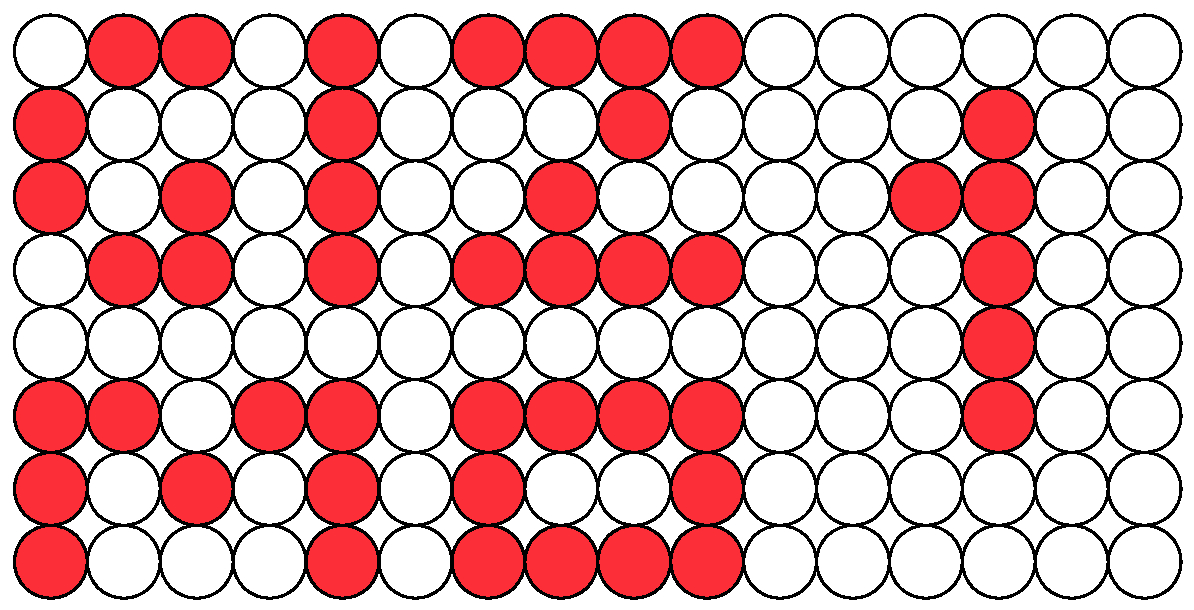
\includegraphics[width=2in]{Gizmo1.pdf}
\vspace{-2em}\caption{\small Boot Screen}\vspace{-2em}
\label{HighLevelGizmoLayout}
\end{wrapfigure}

If you power up Gizmo, or press its reset button, it will display its {\bf boot screen}, which includes the version number (at right, the version number is ``1'').

Gizmo will then show the {\bf root menu}.  Use the left potentiometer to scroll to any of the following applications, and use the select button to select an application.  Available applications are:\,\footnote{Later I'll be adding a {\bf Utility} application, where small MIDI utilities will be available.}

\section {The Arpeggiator}

\begin{wrapfigure}{r}{3in}
\vspace{-1.5em}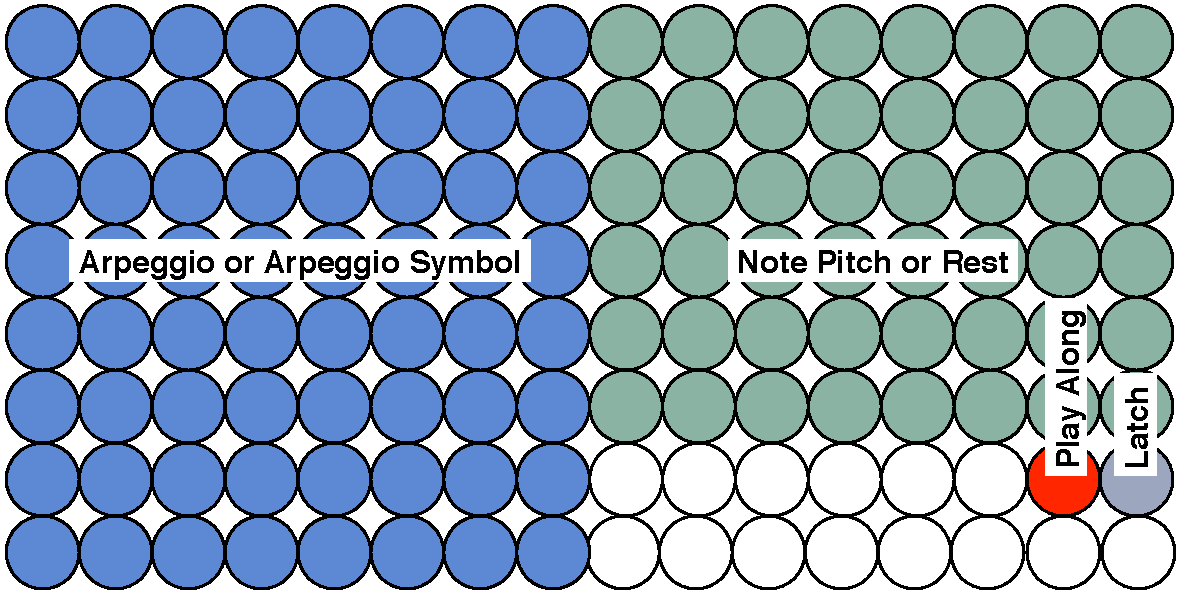
\includegraphics[width=3in]{arpeggio.pdf}
\vspace{-2em}\caption{\small The Arpeggiator Display}\vspace{-1em}
\label{arpeggiator}
\end{wrapfigure}

The arpeggiator allows you to play different kinds of arpeggios, and also to create and save up to ten of them.  The arpeggiator's main menu lets you choose to play five different kinds of pre-set arpeggios, or to select an arpeggio from user-created arpeggio slots 1--10, or finally to create an arpeggio.

An arpeggio is a pattern for repeatedly playing the notes in a chord.  When you hold down a chord on the keyboard, the arpeggiator uses this pattern to play the notes, typically one at a time, according to the pattern selected.  Patterns do not specify exact notes, but rather note orderings.  For example, an arpeggio might be defined as 1, 2, 2, 3, 4, 2, 3: if 1 is set to be the root (lowest) note of your chord, then if you play a C7 chord (C E G B$\flat$), then the arpeggiator will repeat the sequence C E E G B$\flat$ E G.  This pattern will repeat as long as you hold down the keys in the chord.  

Alternatively if you toggle the {\bf latch}, then the playing will continue after you have released the keys, and will only shift to a new chord when you hold down a new chord.  Latch mode is toggled by pressing the Middle button while playing an arpeggio.  When Latch mode is engaged, an LED will light as shown in Figure \ref{arpeggiator}.

\paragraph{Playing Preset Arpeggios}

There are five preset arpeggios: {\it up}, {\it down}, {\it up-down}, {\it chord}, and {\it random}.  

\begin{wrapfigure}{r}{3in}
\begin{center}
\vspace{-1.5em}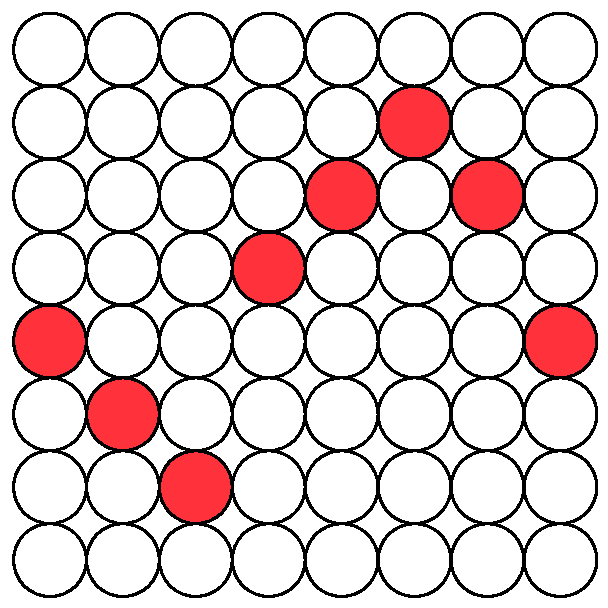
\includegraphics[width=1in]{arpeggioexample.pdf}\\
Example Arpeggio\\[2em]
\vspace{-1.5em}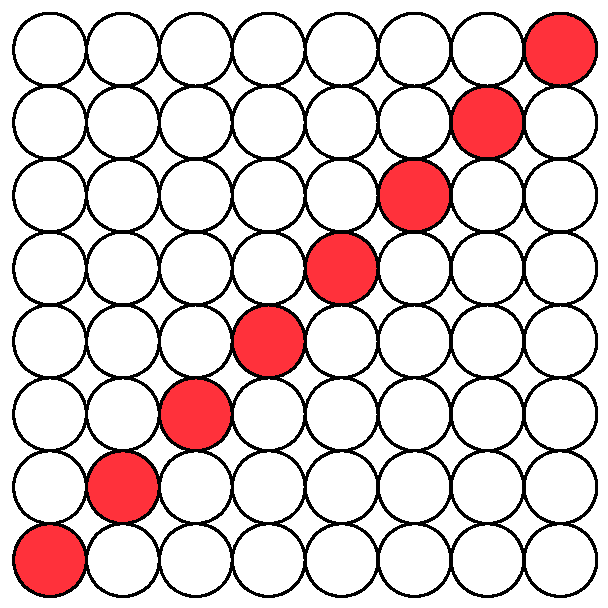
\includegraphics[width=1in]{arpeggioup.pdf}\\
Ascending Notes\\in Sparse Mode\\[2em]
\vspace{-1.5em}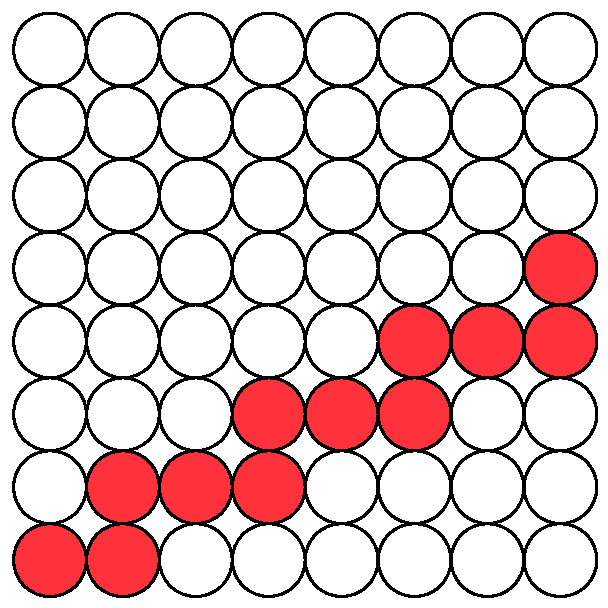
\includegraphics[width=1in]{arpeggiodoubleup.pdf}\\
Ascending Notes\\in Dense Mode\\
\end{center}
\vspace{-2em}\caption{\small General Gauge Display and Frequent MIDI Display}\vspace{-2em}
\label{generalgauge}
\end{wrapfigure}


\section {The Step Sequencer}
\section {The Recorder}
\section {The MIDI Gauge}

\begin{wrapfigure}{r}{3in}
\vspace{-1.5em}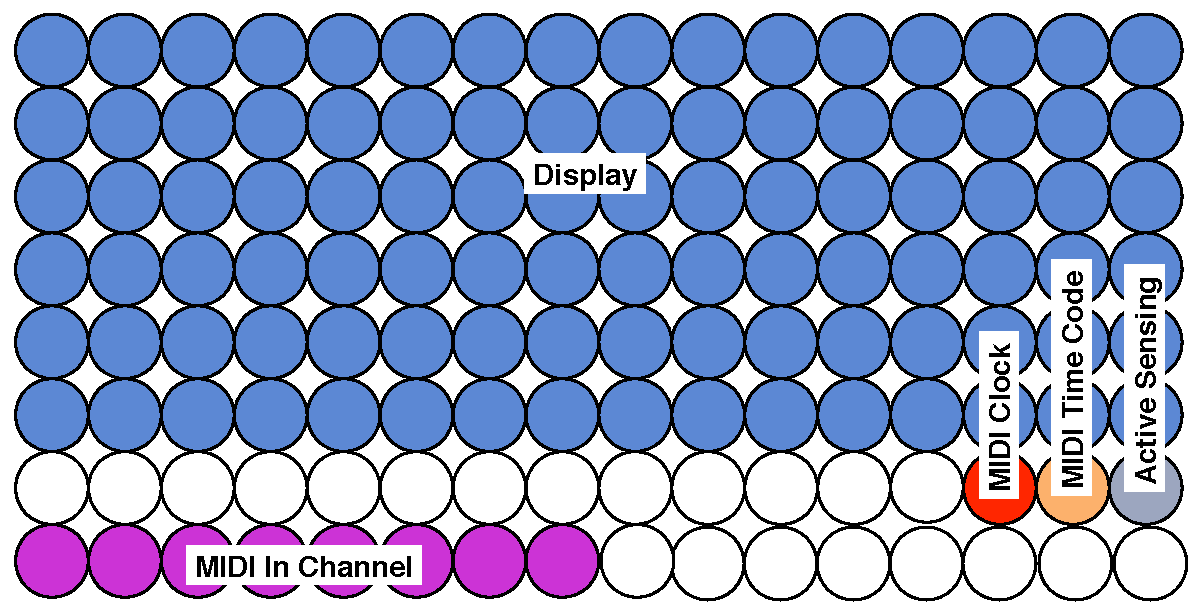
\includegraphics[width=3in]{GeneralGauge.pdf}
\vspace{-2em}\caption{\small General Gauge Display and Frequent MIDI Display}\vspace{-2em}
\label{generalgauge}
\end{wrapfigure}

The MIDI gauge listens to incoming MIDI messages and displays them on-screen.  This only occurs if the MIDI IN channel is something other than NO CHANNEL (See {\bf Options\(\boldsymbol\rightarrow\) In MIDI}, in Section \ref{options}).

\begin{wrapfigure}{r}{2in}
\vspace{-23em}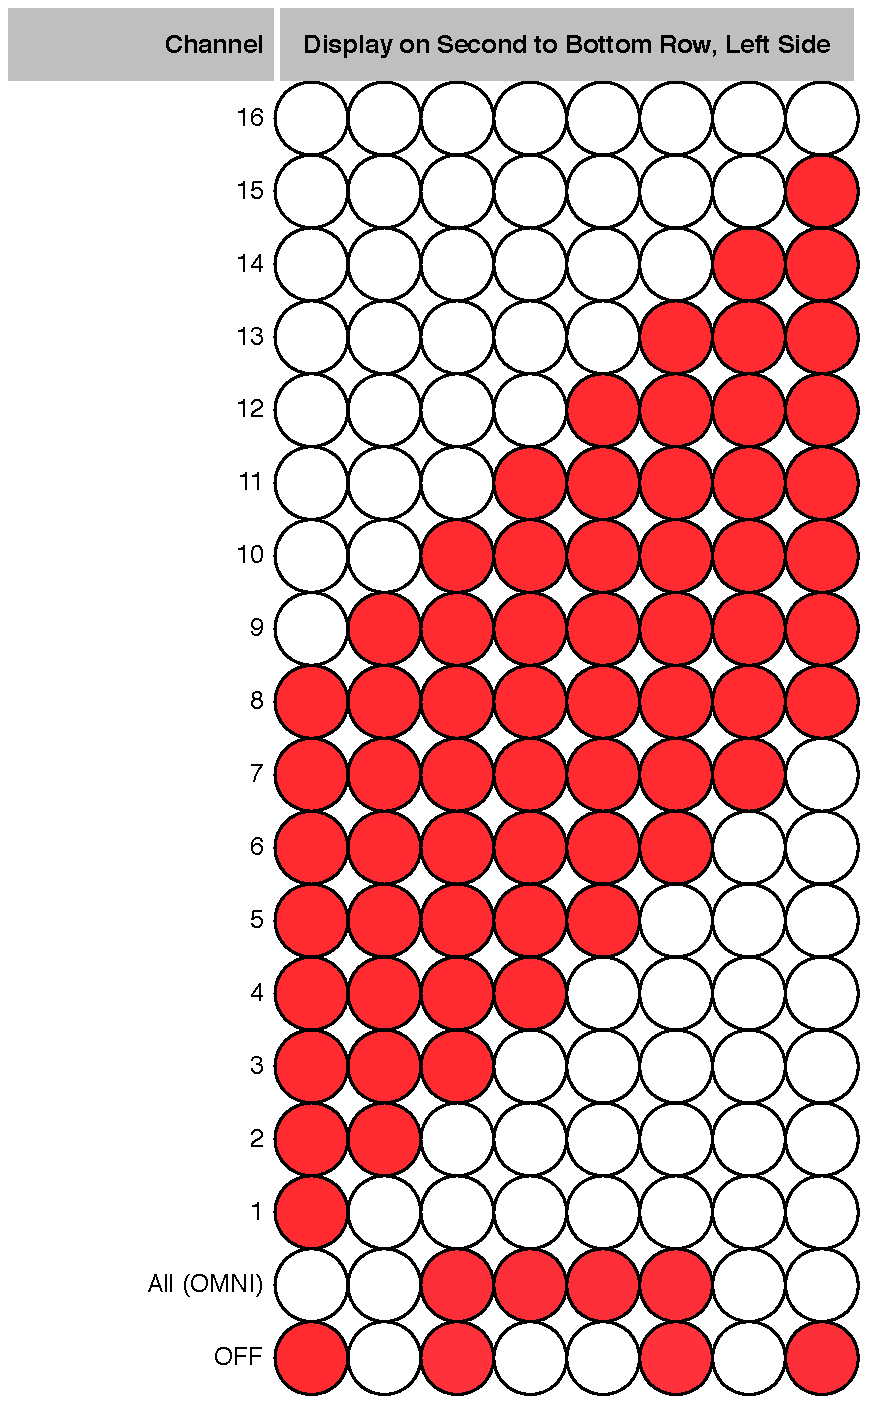
\includegraphics[width=2in]{midichannel.pdf}
\vspace{-2em}\caption{\small MIDI Channel Values}\vspace{-2em}
\end{wrapfigure}


MIDI messages are displayed as follows:  Some MIDI messages are extremely frequent and essentially impossible to display usefully.  





\paragraph{General Gauge Display}  These are simple displays which take up the entire screen.

\begin{itemize}
\item {\bf Pitch Bend}\quad The 14-bit value is displayed
\item {\bf Program Change}\quad ``PC'' is displayed, followed by the value.
\item {\bf Channel Control}\quad Text is scrolled indicating CC, the parameter, and the value.
\item {\bf NRPN}\quad Text is scrolled indicating NRPN, the parameter, and the value (both MSB-only, and MSB+LSB values), plus whether the value was set, incremented, or decremented.
\item {\bf RPN}\quad Text is scrolled indicating NRPN, the parameter, and the value (both MSB-only, and MSB+LSB values), plus whether the value was set, incremented, or decremented.
\item {\bf System Exclusive}\quad ``SYSX'' is displayed.
\item {\bf Song Position}\quad ``SPOS'' is displayed.
\item {\bf Song Select}\quad ``SSEL'' is displayed.
\item {\bf Tune Request}\quad ``TREQ'' is displayed.
\item {\bf Start}\quad ``STRT'' is displayed.
\item {\bf Continue}\quad ``CONT'' is displayed.
\item {\bf Stop}\quad ``STOP'' is displayed.
\item {\bf System Reset}\quad ``RSET'' is displayed.
\end{itemize}

\paragraph{Frequent MIDI Display}  These are messages which are too fast to display usefully in most cases.  In each case, a specific LED will be toggled (see Figure \ref{generalgauge}).

\paragraph{}\vspace{-2em}\begin{itemize}
\item {\bf Active Sensing}
\item {\bf MIDI Time Code}
\item {\bf MIDI Clock}
\item {\bf Channel Aftertouch}.  This one is special.  If you press the {\bf middle button}, you can toggle whether aftertouch is displayed as a simple toggled LED, or if the display should say ``AT'', followed by the aftertouch value.
\end{itemize}

\begin{wrapfigure}{r}{3in}
\vspace{-1.5em}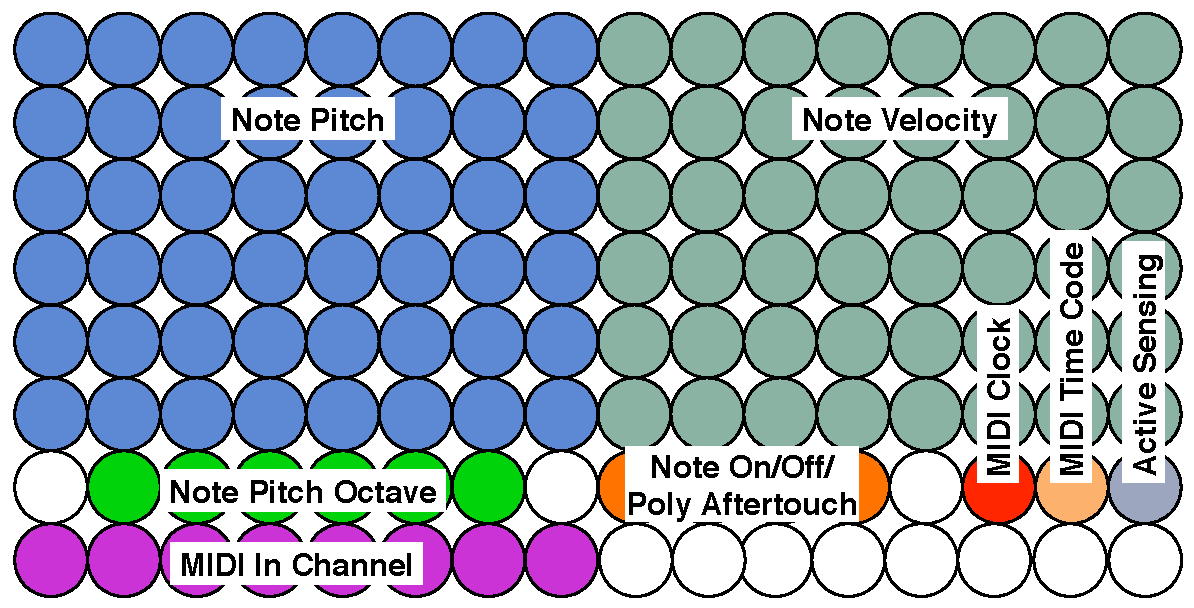
\includegraphics[width=3in]{NoteGauge.pdf}
\vspace{-2em}\caption{\small Note Gauge Layout}\vspace{-1em}
\label{notegauge}
\end{wrapfigure}

\paragraph{Note Display}

Note messages are displayed with both the {\bf pitch} (at left) and the {\bf velocity} (at right) of the note value, plus the particular kind of message in question: {\bf Note On, Note Off,} and {\bf Polyphonic Aftertouch}.

Polyphonic Aftertouch is special.  If you press the {\bf middle button}, you can toggle whether aftertouch is displayed as a simple toggled LED (along with Channel Aftertouch), or if the aftertouch information should be displayed like the Note On/Off data.

\begin{wrapfigure}{r}{1.6in}
\vspace{1em}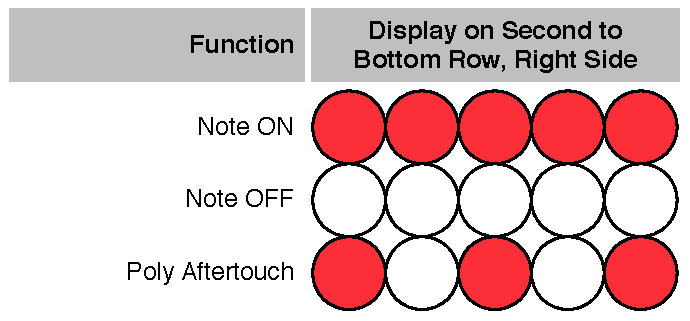
\includegraphics[width=1.6in]{notefunction.pdf}
\vspace{-2em}\caption{\small Note Function}\vspace{-1em}
\label{notefunction}
\end{wrapfigure}

How do you distinguish between a Note On, Note Off, or Polyphonic Aftertouch message?  Figure \ref{notegauge} shows a four-LED region, in orange, where a certain pattern is displayed to indicate this.  The patterns are shown in Figure \ref{notefunction}/

\begin{wrapfigure}{r}{1.8in}
\vspace{1em}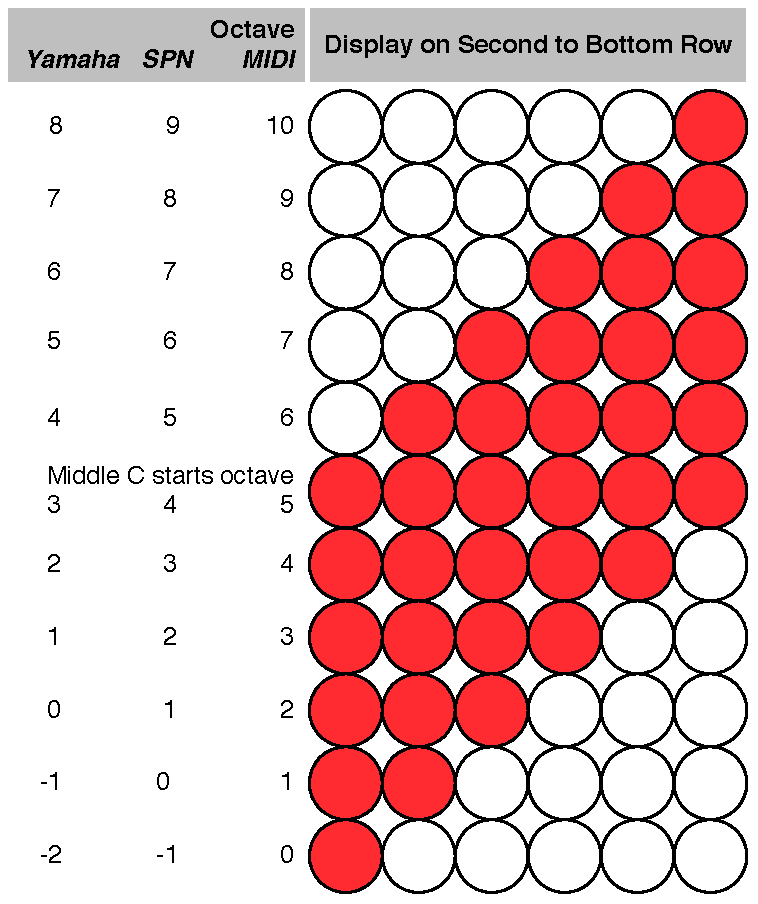
\includegraphics[width=1.8in]{octave.pdf}
\vspace{-2em}\caption{\small Octave Values}\vspace{-1em}
\label{octave}
\end{wrapfigure}

Note pitches are displayed by showing the note (such as B$\flat$), with the octave number directly below it.  MIDI has eleven different octaves (0--10): Middle C is the bottom note of octave 5.  The octave number is displayed as shown in Figure \ref{octave}.  As usual, the MIDI In Channel is shown below that.


\section {The Controller}

The Controller allows you to assign to each of two buttons and two potentiometers any NRPN, RPN, Control Change (CC), or Program Change (PC) value.  These assignments are stored in Flash memory and survive reboots and power cycling.

	\begin{description}

	\item{\bf Go}
	
	This enters the controller proper.  Turning the left or right knobs, or pressing the Select or Middle buttons, will cause them to issue MIDI messages as assigned (below).  If you press the Back button, you can exit the controller.
	
	When you turn a knob or press a button, and the knob/button has had its control type set to something other than OFF, then the appropriate MIDI message is sent, and the value of the message is displayed as a number on-screen.  Messages are only sent if the MIDI OUT channel is something other than NO CHANNEL (See {\bf Options\(\boldsymbol\rightarrow\) Out MIDI}, in Section \ref{options}).
	
	Note that for the time being the controller will only send (MSB) values between 0...127.  It cannot send 14-bit NRPN and RPN values.  This is largely a limitation of the resolution of the potentiometers.

	\item{\bf Left Knob}
	
	This submenu lets you select your control type and parameter number for the left potentiometer.
	
	You are first given the option of what kind of {\bf control type} (OFF, CC, NRPN, RPN, PC) you would like to manipulate with the left knob.  If OFF, then turning the knob will not do anything.

	After you have selected a control type, if you have selected CC, NRPN, or RPN, you will be then asked to select a {\bf controller parameter number}.  (Otherwise ,for PC and OFF, you will go back to the top-level Controller Menu).  CC parameter numbers may range 0 ... 119.  NRPN and RPN parameter numbers may range 0 ... 16383. When you have completed this, you will be sent back to the top-level Controller menu.

	\item{\bf Right Knob}
	
	This submenu lets you select your control type and parameter number for the right potentiometer.
	
	You are first given the option of what kind of {\bf control type} (OFF, CC, NRPN, RPN, PC) you would like to manipulate with the right knob.  If OFF, then turning the knob will not do anything.

	After you have selected a control type, if you have selected CC, NRPN, or RPN, you will be then asked to select a {\bf controller parameter number}.  (Otherwise ,for PC and OFF, you will go back to the top-level Controller Menu).  CC parameter numbers may range 0 ... 119.  NRPN and RPN parameter numbers may range 0 ... 16383. When you have completed this, you will be sent back to the top-level Controller menu.
	
	\item{\bf Middle Button}
	
	This submenu lets you select your control type, parameter number, and on/off values for the middle button.
	
	You are first given the option of what kind of {\bf control type} (OFF, CC, NRPN, RPN, PC) you would like to manipulate with the middle button.  If OFF, then pressing the button will not do anything.

	After you have selected a control type, if you have selected CC, NRPN, or RPN, you will be then asked to select a {\bf controller parameter number}.  (Otherwise ,for PC and OFF, you will go back to the top-level Controller Menu).  CC parameter numbers may range 0 ... 119.  NRPN and RPN parameter numbers may range 0 ... 16383.
	
	When you have completed this, you will be then asked to enter the value sent when the button is {\bf pressed}.  This value must be 0...127 (the Controller does not send 14-bit values).  Afterwards, you will be similarly asked to enter the value sent when the button is {\bf pressed again} (the buttons act as toggles).  When you have completed this, you will be sent back to the top-level Controller menu.

	\item{\bf Select Button}
	
	This submenu lets you select your control type, parameter number, and on/off values for the select button.
	
	You are first given the option of what kind of {\bf control type} (OFF, CC, NRPN, RPN, PC) you would like to manipulate with the select button.  If OFF, then pressing the button will not do anything.

	After you have selected a control type, if you have selected CC, NRPN, or RPN, you will be then asked to select a {\bf controller parameter number}.  (Otherwise ,for PC and OFF, you will go back to the top-level Controller Menu).  CC parameter numbers may range 0 ... 119.  NRPN and RPN parameter numbers may range 0 ... 16383.
	
	When you have completed this, you will be then asked to enter the value sent when the button is {\bf pressed}.  This value must be 0...127 (the Controller does not send 14-bit values).  Afterwards, you will be similarly asked to enter the value sent when the button is {\bf pressed again} (the buttons act as toggles).  When you have completed this, you will be sent back to the top-level Controller menu.

	\end{description}

\section {Options}
\label{options}

	Options sets global parameters for the device.  Once set, these parameters are stored in Flash memory and so will survive a power cycle.  Some options can be also accessed from certain other applications as a convenience.  
	
	\begin{description}


	\item{\bf Tempo}\\
	If Gizmo is following its own internal clock rather than relying on an external MIDI clock , this specifies how fast a quarter note is.  If Gizmo is following an external MIDI clock, this value is ignored, and the MIDI clock's specification of a quarter note is used instead.  (See {\bf Options\(\boldsymbol\rightarrow\)MIDI~Clock}).  When not in {\bf Bypass Mode}, the tempo is shown by the pulsing on/off of the {\bf Beat / Bypass Light} (see Figure \ref{HighLevelGizmoLayout}). 
	
		\begin{description}
		\item{\bf \textit{Choose}}: 1 ... 999 Beats Per Minute.  Note that this is a large number, and so may require you to choose it with the left potentiometer, then fine-tune it with the right potentiometer.\footnote{Gizmo can go lots faster than 999: in theory it could go clear to 31200 or so.  But then your synthesizer would explode and we wouldn't want that.}
		\end{description}
		
	\item{\bf Note Speed}\\
		Various applications (arpeggiators, step sequencers)
		produce notes at a certain rate relative to the tempo.
		For example, though the tempo may specify that a
		quarter note is set to 120 Beats Per Minute, the 
		arpeggiator might be generating eighth notes and
		so is producing notes at twice that speed.  You specify the 
		note speed here.
		
		Note speed is shown by pulsing the {\bf Note Pulse Light} (Figure \ref{HighLevelGizmoLayout}).

		\begin{description}
			\item{\bf \textit{Choose}}:
			\begin{tabbing}
			Eighth Triplet\hspace{10em}\=\(\myfrac{1}{24}\)\hspace{1em}\=Beat\\
			Quarter Triplet\>\(\myfrac{1}{12}\)\>Beat\\
			Thirty-Second Note\>\(\myfrac{1}{8}\)\>Beat\hspace{0.7in}\=\smash{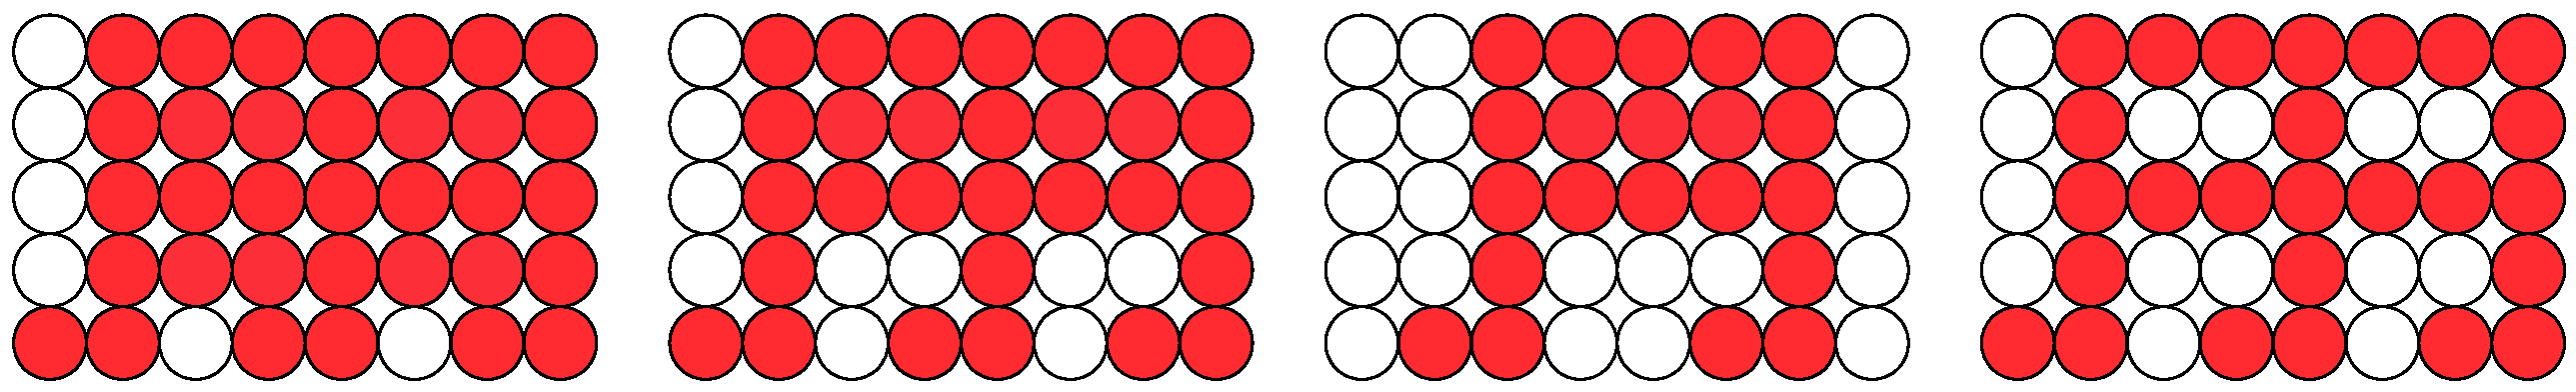
\includegraphics[width=2in]{NoteSpeed1.pdf}}\\
			Half Triplet\>\(\myfrac{1}{6}\)\>Beat\\
			\\
			Sixteenth Note\>\(\myfrac{1}{4}\)\>Beat\\
			Triplet\>\(\myfrac{1}{3}\)\>Beat\\
			Eighth Note\>\(\myfrac{1}{2}\)\>Beat\>\smash{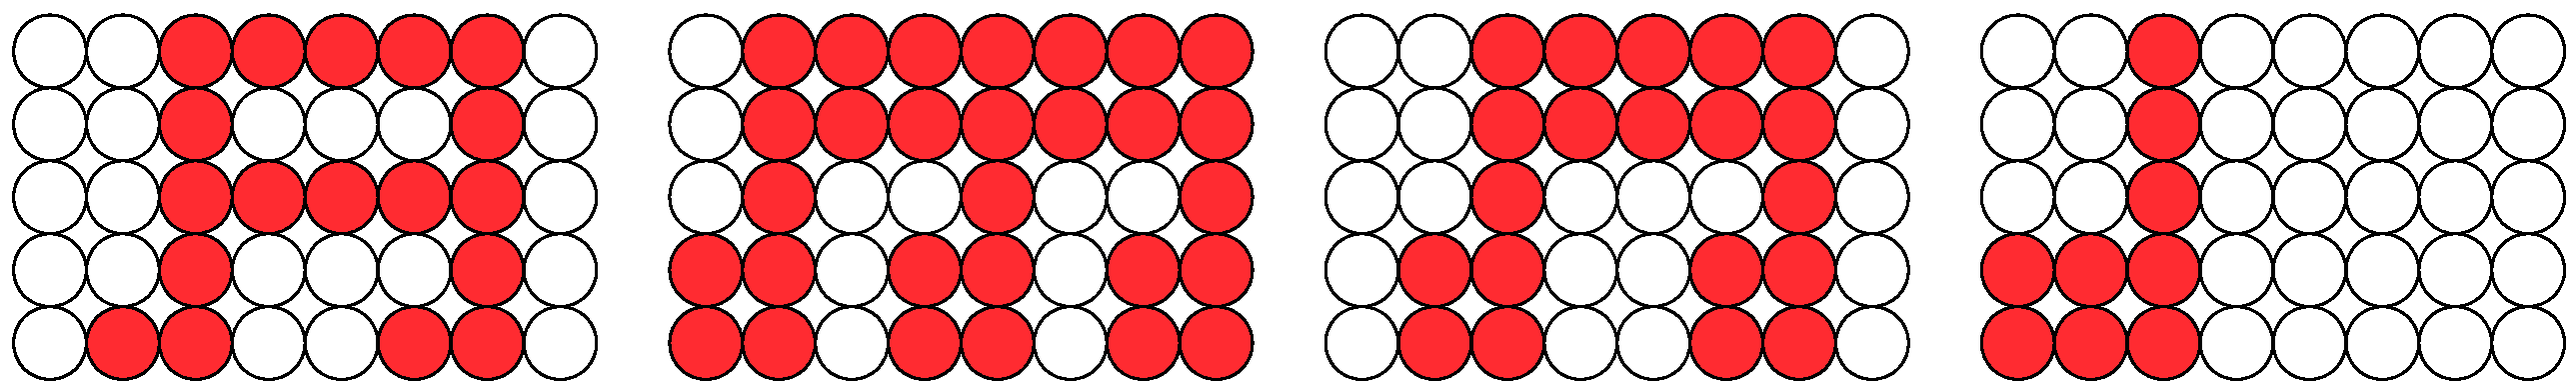
\includegraphics[width=2in]{NoteSpeed2.pdf}}\\
			Quarter Note\>\(1\)\>Beat (duh)\\
			\\
			Quarter Note Tied to Triplet\>\(1\ \, \myfrac{1}{3}\)\>Beats\\
			Dotted Quarter Note\>\(1\ \, \myfrac{1}{2}\)\>Beats\\
			Half Note\>\(2\)\>Beats\>\smash{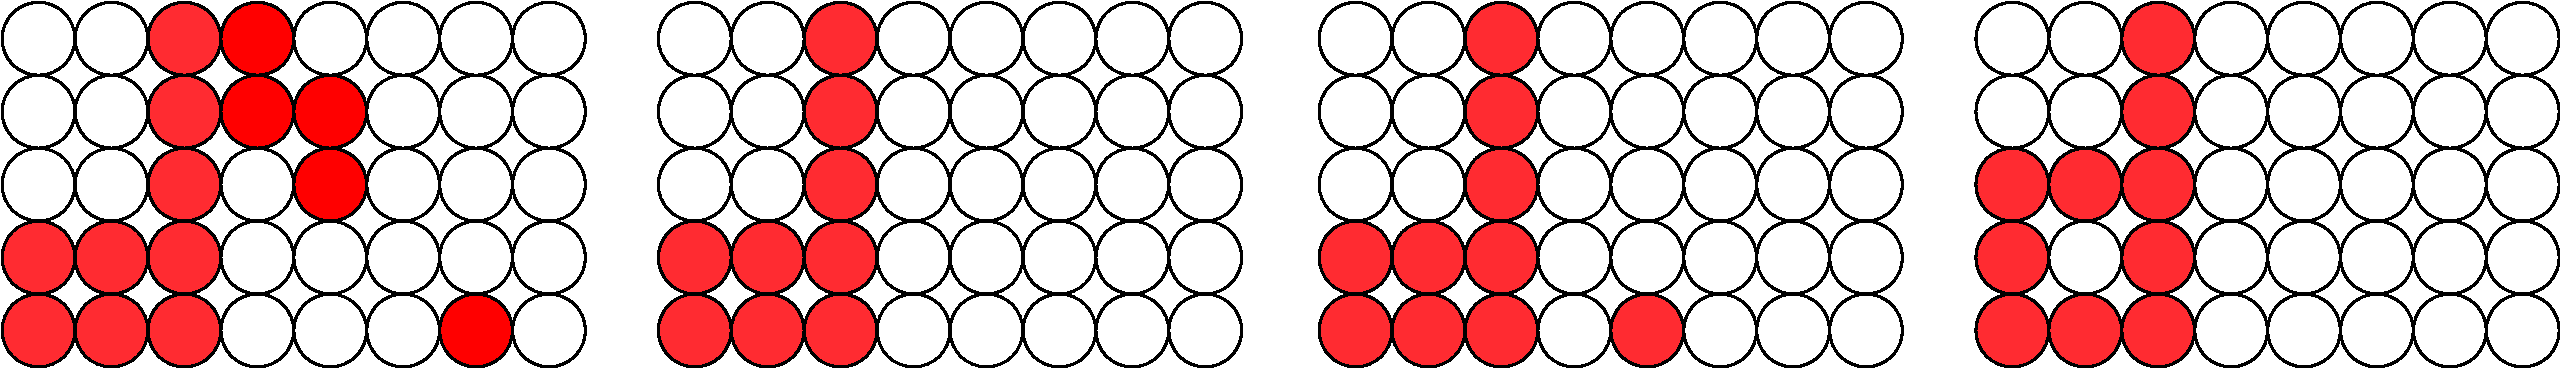
\includegraphics[width=2in]{NoteSpeed3.pdf}}\\
			Half Note Tied to Two Triplets\>\(2\ \, \myfrac{2}{3}\)\>Beats\\
			\\
			Dotted Half Note\>\(3\)\>Beats\\
			Whole Note\>\(4\)\>Beats\\
			Dotted Whole Note\>\(6\)\>Beats\>\smash{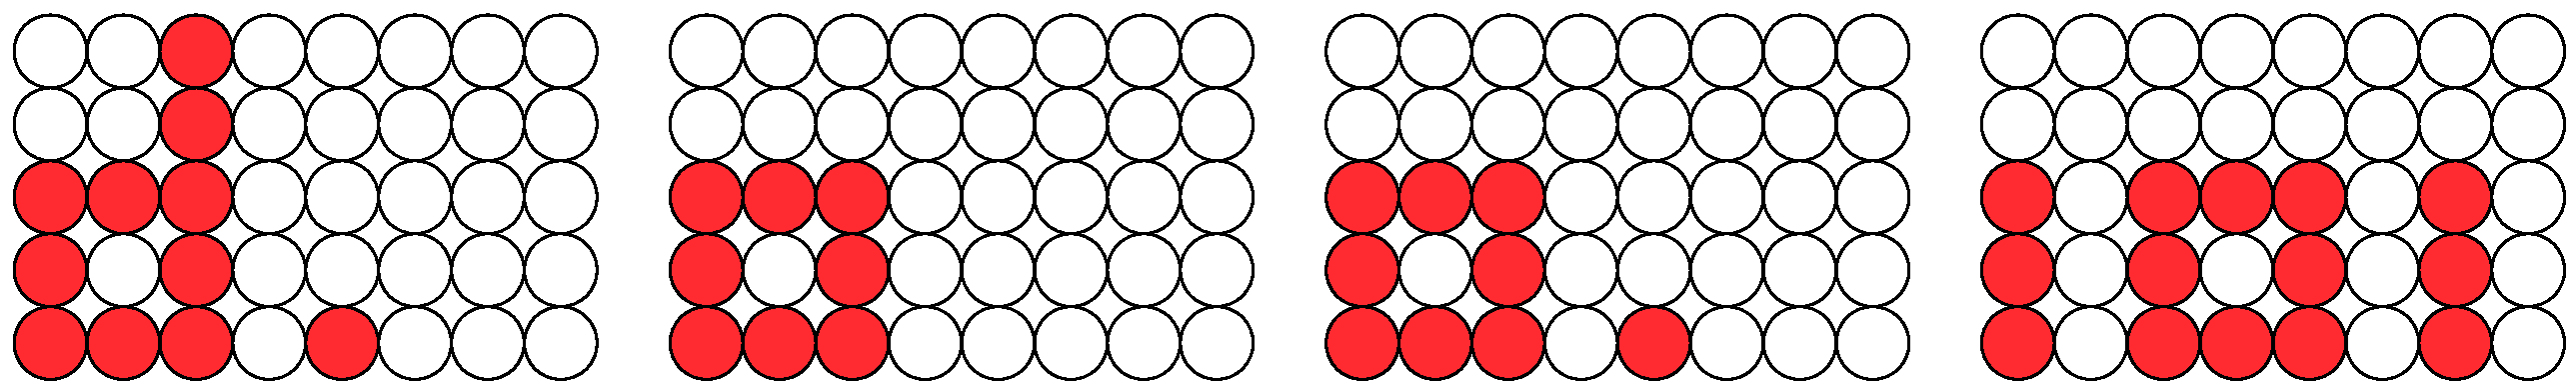
\includegraphics[width=2in]{NoteSpeed4.pdf}}\\
			Double Whole Note\>\(8\)\>Beats
			\end{tabbing}
		\end{description}

	\item{\bf Swing}\\
			Swing, or {\bf syncopation}, is the degree to which every even eighth note is delayed.  0\% means no swing at all.  100\% means so much swing that the even note plays at the same time as the next even eighth note.  That's a lot.
		\begin{description}
		\item{\bf \textit{Choose}}: 0\% ... 100\% (larger percentages are more swing, that is, longer delay every other note)
		\end{description}


	\item{\bf Transpose}\\
		Here you can state that any notes generated by Gizmo be {\bf transposed} up or down by as much as 60 notes. If a note is transposed to the point that it exceeds the MIDI range, it is not played.  When appropriate, some applications (such as the MIDI Gauge) ignore this option. 
		\begin{description}
		\item{\bf \textit{Choose}}: \(-60\) ... 60 
		\end{description}

	\item{\bf Volume}\\
		Like Transpose, here you can state that any notes generated by Gizmo have their volume changed by multiplying their MIDI velocity by some value.  If a resulting note velocity exceeds the maximum (127), it is bounded to 127.
			
			\begin{description}
			\item{\bf \textit{Choose}}:
			\begin{tabbing}
			1/8\\
			1/4\\
			1/2\hspace{3.65in}\smash{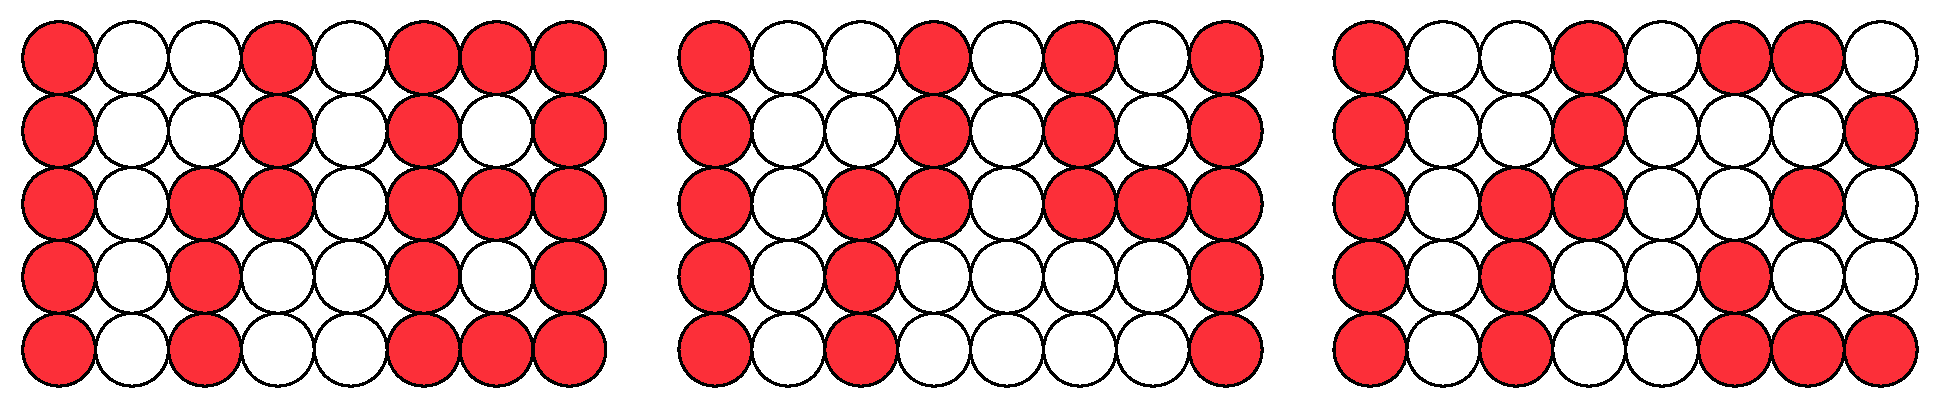
\includegraphics[width=1.7in]{fractions2.pdf}}\\
			1(default)\\
			2\\
			4\\
			8\\
			\end{tabbing}
		\end{description}

	\item{\bf In MIDI}\,\footnote{{\it Why aren't these called MIDI In and MIDI Out?}  Because then they'd be indistinguishable on the menu screen before the text started scrolling.}\\
		Many applications expect notes and other controls to come in via a specific input MIDI channel.  You specify it here.
		\begin{description}
		\item{\bf \textit{Choose}}: No Channel, Channels 1...16, or ALL Channels\hspace{0.25in}\smash{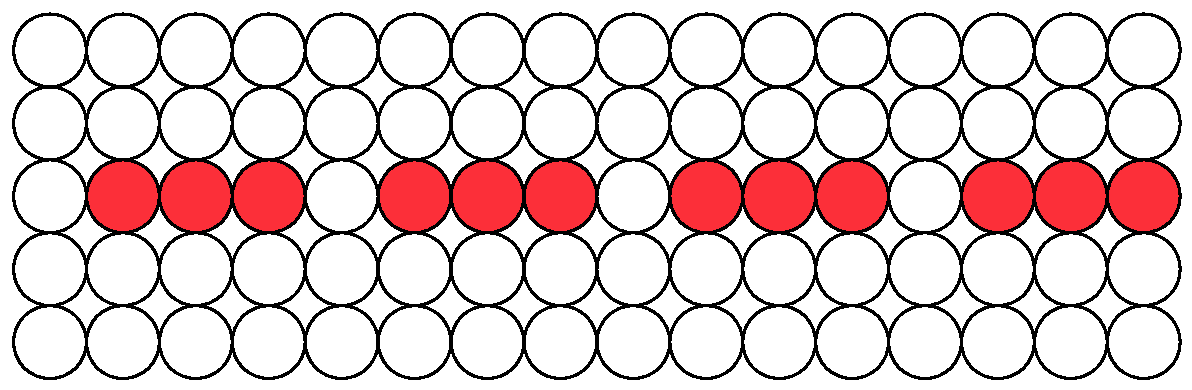
\includegraphics[width=1in]{none.pdf}}\hspace{0.2in}\smash{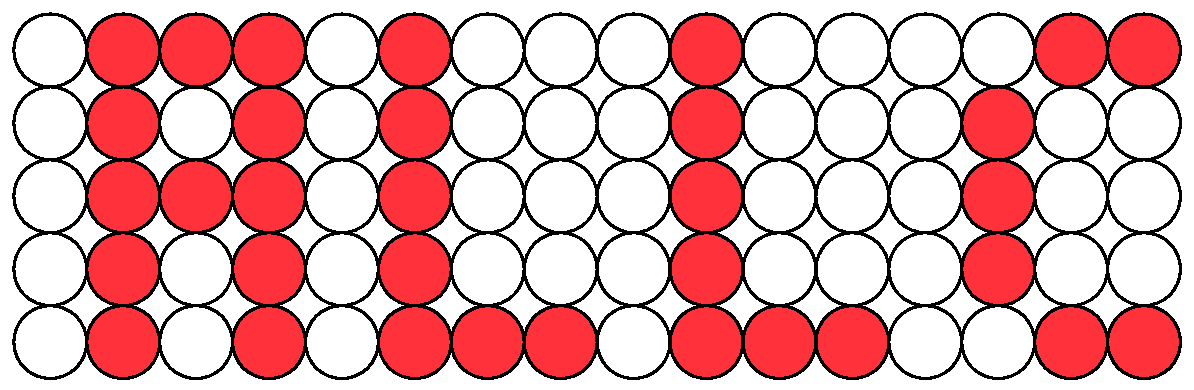
\includegraphics[width=1in]{all.pdf}}\\
		\end{description}
	\item{\bf Out MIDI}
		Many applications emit notes etc. via a specific output MIDI channel.  You specify it here.  Other applications can emit notes on several different channels, in which case this value determines the default channel used.
		\begin{description}
		\item{\bf \textit{Choose}}: No Channel, or Channels 1...16\hspace{0.5in}\smash{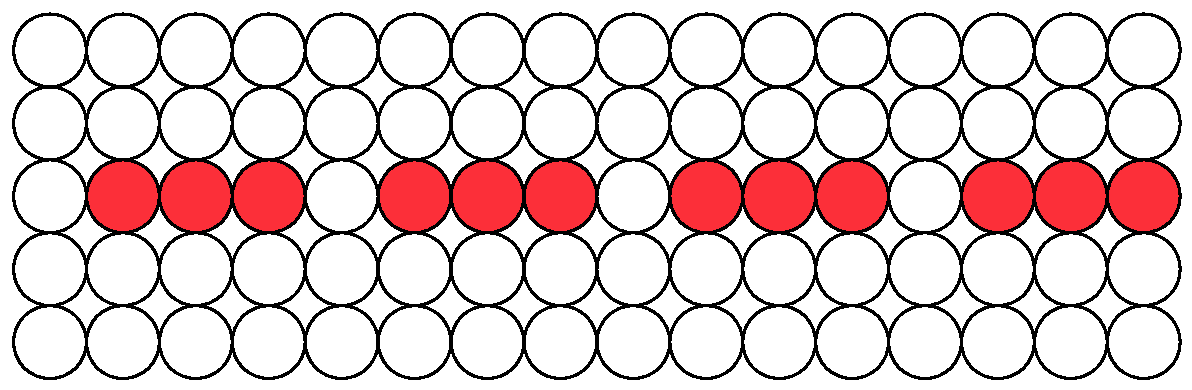
\includegraphics[width=1in]{none.pdf}}
		\end{description}
	\item{\bf Control MIDI}\\
		The arduino can be controlled via NRPN messages.  You specify the channel here on which it will listen for them
		\begin{description}
		\item{\bf \textit{Choose}}: No Channel, or Channels 1...16\hspace{0.5in}\smash{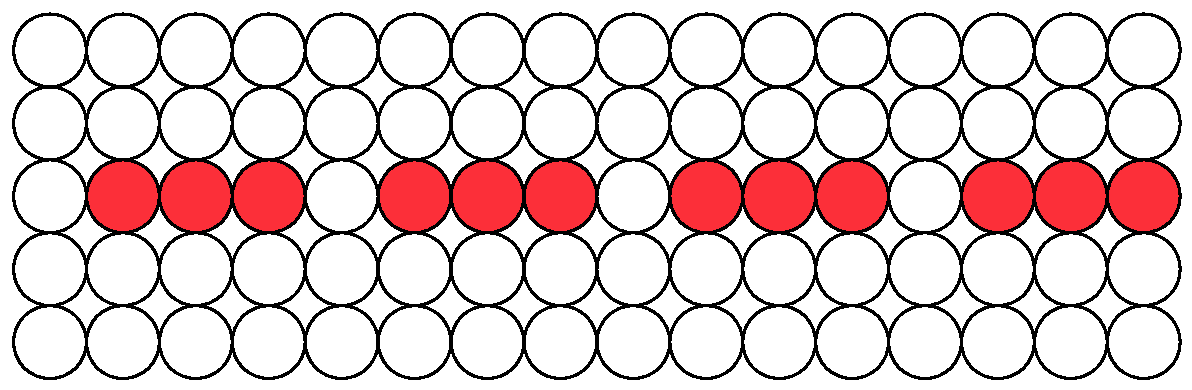
\includegraphics[width=1in]{none.pdf}}
		\end{description}
		
		The NRPN Messages are:
		
		\noindent\begin{tabular}{@{}rlllp{2.4in}@{}}
		{\it NRPN Parameter}&{\it Min  Value}&{\it Max Value}&{\it MSB/LSB}&{\it Description}\\[0.1em]
		\hline\\[-0.9em]
		0	&0 (released)	&1 (pressed) & MSB& Press/Release the Back Button\\
		1	&0 (released)	&1 (pressed) & MSB & Press/Release the Middle Button\\
		2	&0 (released)	&1 (pressed) & MSB & Press/Release the Select Button\\
		3	&0	& 1023 & MSB + LSB & Turn the Left Potentiometer\\
		4	&0	& 1023 & MSB + LSB & Turn the Right Potentiometer\\
		5	&0 (un-bypass)	&1 (bypass) & MSB& Toggle Bypass\\
		6	& Any Value &Any Value & MSB& Unlock Potentiometers.  When an NRPN message is received, normally the on-board potentiometers are locked so that turning them has no effect.  Pressing an on-board button unlocks them: so does sending this NRPN message.\\
		7	&	Any Value &Any Value & MSB& Start Clock.  If Gizmo's clock is stopped, resets and starts it.  When appropriate, sends a MIDI START message.\\
		8	& Any Value	&Any Value & MSB& Stop Clock.  If Gizmo's clock is playing, stops it.  When appropriate, sends a MIDI STOP message.\\
		9	&	Any Value &Any Value & MSB & Continue Clock.    If Gizmo's clock is stopped, continues it.  When appropriate, sends a MIDI CONTINUE message.\\
		
		
		\end{tabular}
		
	\item{\bf MIDI Clock}\\
		Gizmo can respond to a MIDI clock, ignore it, or emit its own MIDI clock.  The use of the {\bf Options\(\boldsymbol\rightarrow\)Tempo} setting will depend on the setting chosen here.
		\begin{description}
			\item{\bf \textit{Choose}}:
			\begin{tabbing}
			Ignore\hspace{0.5in}\=Use an internal clock but let any external MIDI clock pass through.\\
			Use\>Use an external MIDI clock and also let it pass through.\\
			Consume\>Use an external MIDI clock but don't let it pass through.\\
			Generate\>Use an internal clock and emit it as a MIDI clock.\\
			\>~~~~~~Don't let any external MIDI clock pass through.\\	
			Block\>Use an internal clock but don't emit as a MIDI clock.\\
			\>~~~~~~Don't let any external MIDI clock pass through.\\
			\end{tabbing}
		\end{description}

	\item{\bf Screen Brightness}\\
		This changes the brightness of the LED matrix.
		\begin{description}
		\item{\bf \textit{Choose}}: 1...16 (higher values are brighter)
		\end{description}
	\item{\bf Menu Delay}\\
		Gizmo often will display text (such as ``SWING'') by filling the screen with the first few letters (in this case, ``SWI''), then pausing for a certain delay, then scrolling through the whole word horizontally. You can specify how long that pause is here.
		\begin{description}
			\item{\bf \textit{Choose}}:
			\begin{tabbing}
			0\hspace{2em}\=Seconds\hspace{1in}\=(scroll immediately)\\
			1/8\>Seconds\\
			1/4\>Seconds\\
			1/3\>Seconds\>\hspace{1.5in}\=\smash{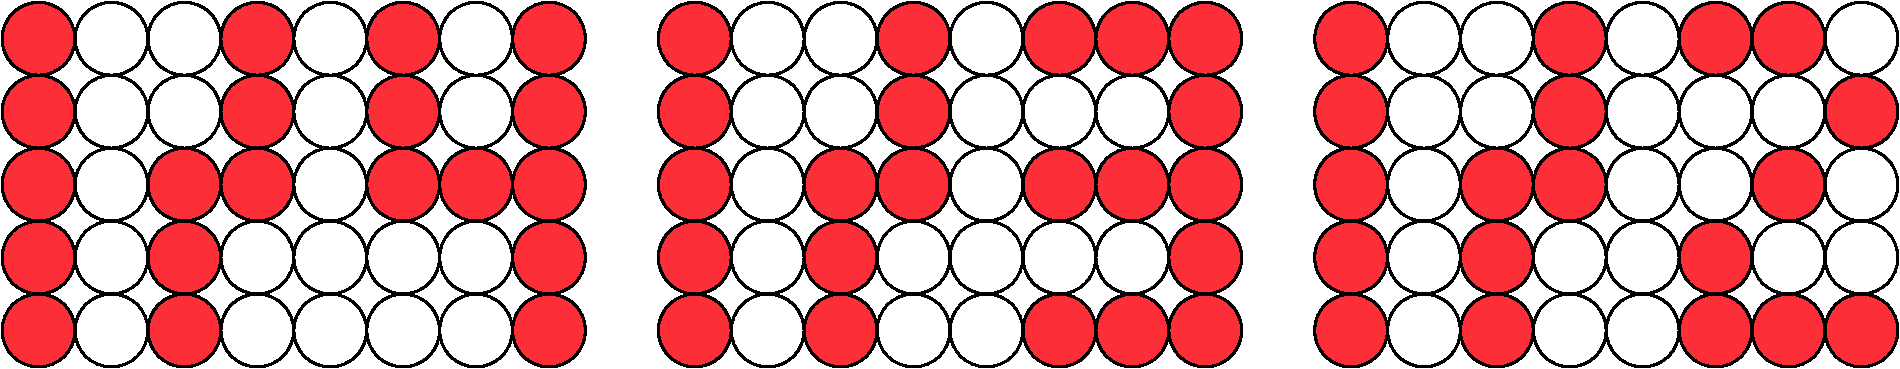
\includegraphics[width=2in]{fractions.pdf}}\\
			1/2\>Seconds\\
			1\>Second\>(default)\\
			2\>Seconds\\
			3\>Seconds\\
			4\>Seconds\\
			8\>Seconds\\
			\(\infty\)\>Seconds\>(never scroll)\>\smash{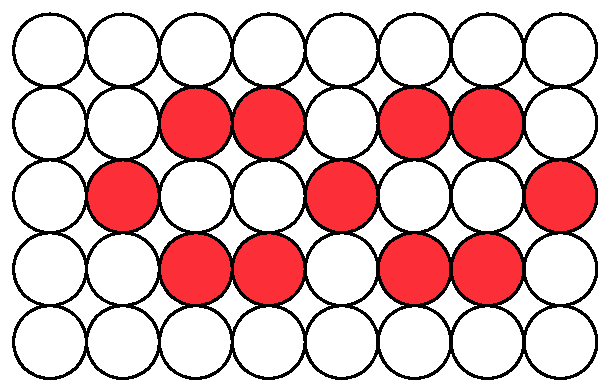
\includegraphics[width=0.48in]{infinity}}\\
			\end{tabbing}
		\end{description}
%	\item{\bf Voltage} (or {\bf No Voltage)}\\
%		Toggles whether Gizmo will send voltage information out via the optional DACs in response to notes played or to Controller potentiometers being turned.  
	\item{\bf The About Screen}\\
		Presently says:\quad GIZMO V1 (C) 2016 BY SEAN LUKE
	\item{\bf Starting, Stopping, and Continuing the Clock}
		This isn't a menu option.  But if you are in the Options menu, you can control the clock:  pressing the Middle Button will {\bf start} or {\bf stop} the clock.  Long-pressing 
	\end{description}

\end{document}
